In this chapter the website and it's functions are described. Furthermore, there will be some explanation about the logic that drives the website.

\section{Reason of existence}
The website is the place where the online speakers and objects are manipulated.
The idea of the website is to enable the user to simply drag and drop speakers/objects with platform independency in mind.
The website had to be simple, easy to use and not dependent of some kind of webserver.
So the website has to be portable\footnote{Platform independent, eg usable on Linux, Windows, etc...}.
For this reason the website's main logic is made in JavaScript and The layout with simple HTML and a small hint of CSS which was used to bring it all up to flavor.
Most web browser's can open the website, the \textit{index.html} file, and see the site and online speakers.

\section{Challenges}
Some challenges that where faced when making this website. Some where small and some where big. {\tiny\textit{Insert Yo Momma Joke}}

\subsection{MQTT with web sockets}
This website needs to connect to an MQTT broker. Because of the rule of platform independency and portability, some kind of connectivity with JavaScript is needed.
Enter the world of web sockets! For this project, the \href{https://github.com/eclipse/paho.mqtt.javascript}{Paho JavaScript Client} is used.
The Paho JavaScript Client is an MQTT browser-based client library written in JavaScript that uses Web Sockets to connect to an MQTT Broker.
This implementations still has some limits\footnotemark, but for this project it was doing it's job quite well.
\footnotetext{When dealing wit non Unicode characters, the client will crash. This was addressed apparently in some fork of the client, but not in this implementation.}

\subsection{Website flow}
In figure \ref{fig:website_flow} is the startup and flow sequence of the website displayed.
When the site comes online, the unknown dataset\footnotemark first has to be rebuild.
\footnotetext{The dataset is all the online clients with all the objects and their information. See \hyperref[clients]{clients} of the \hyperref[chap:Topics]{topics chapter}}

\begin{figure}[H]
    \centering
    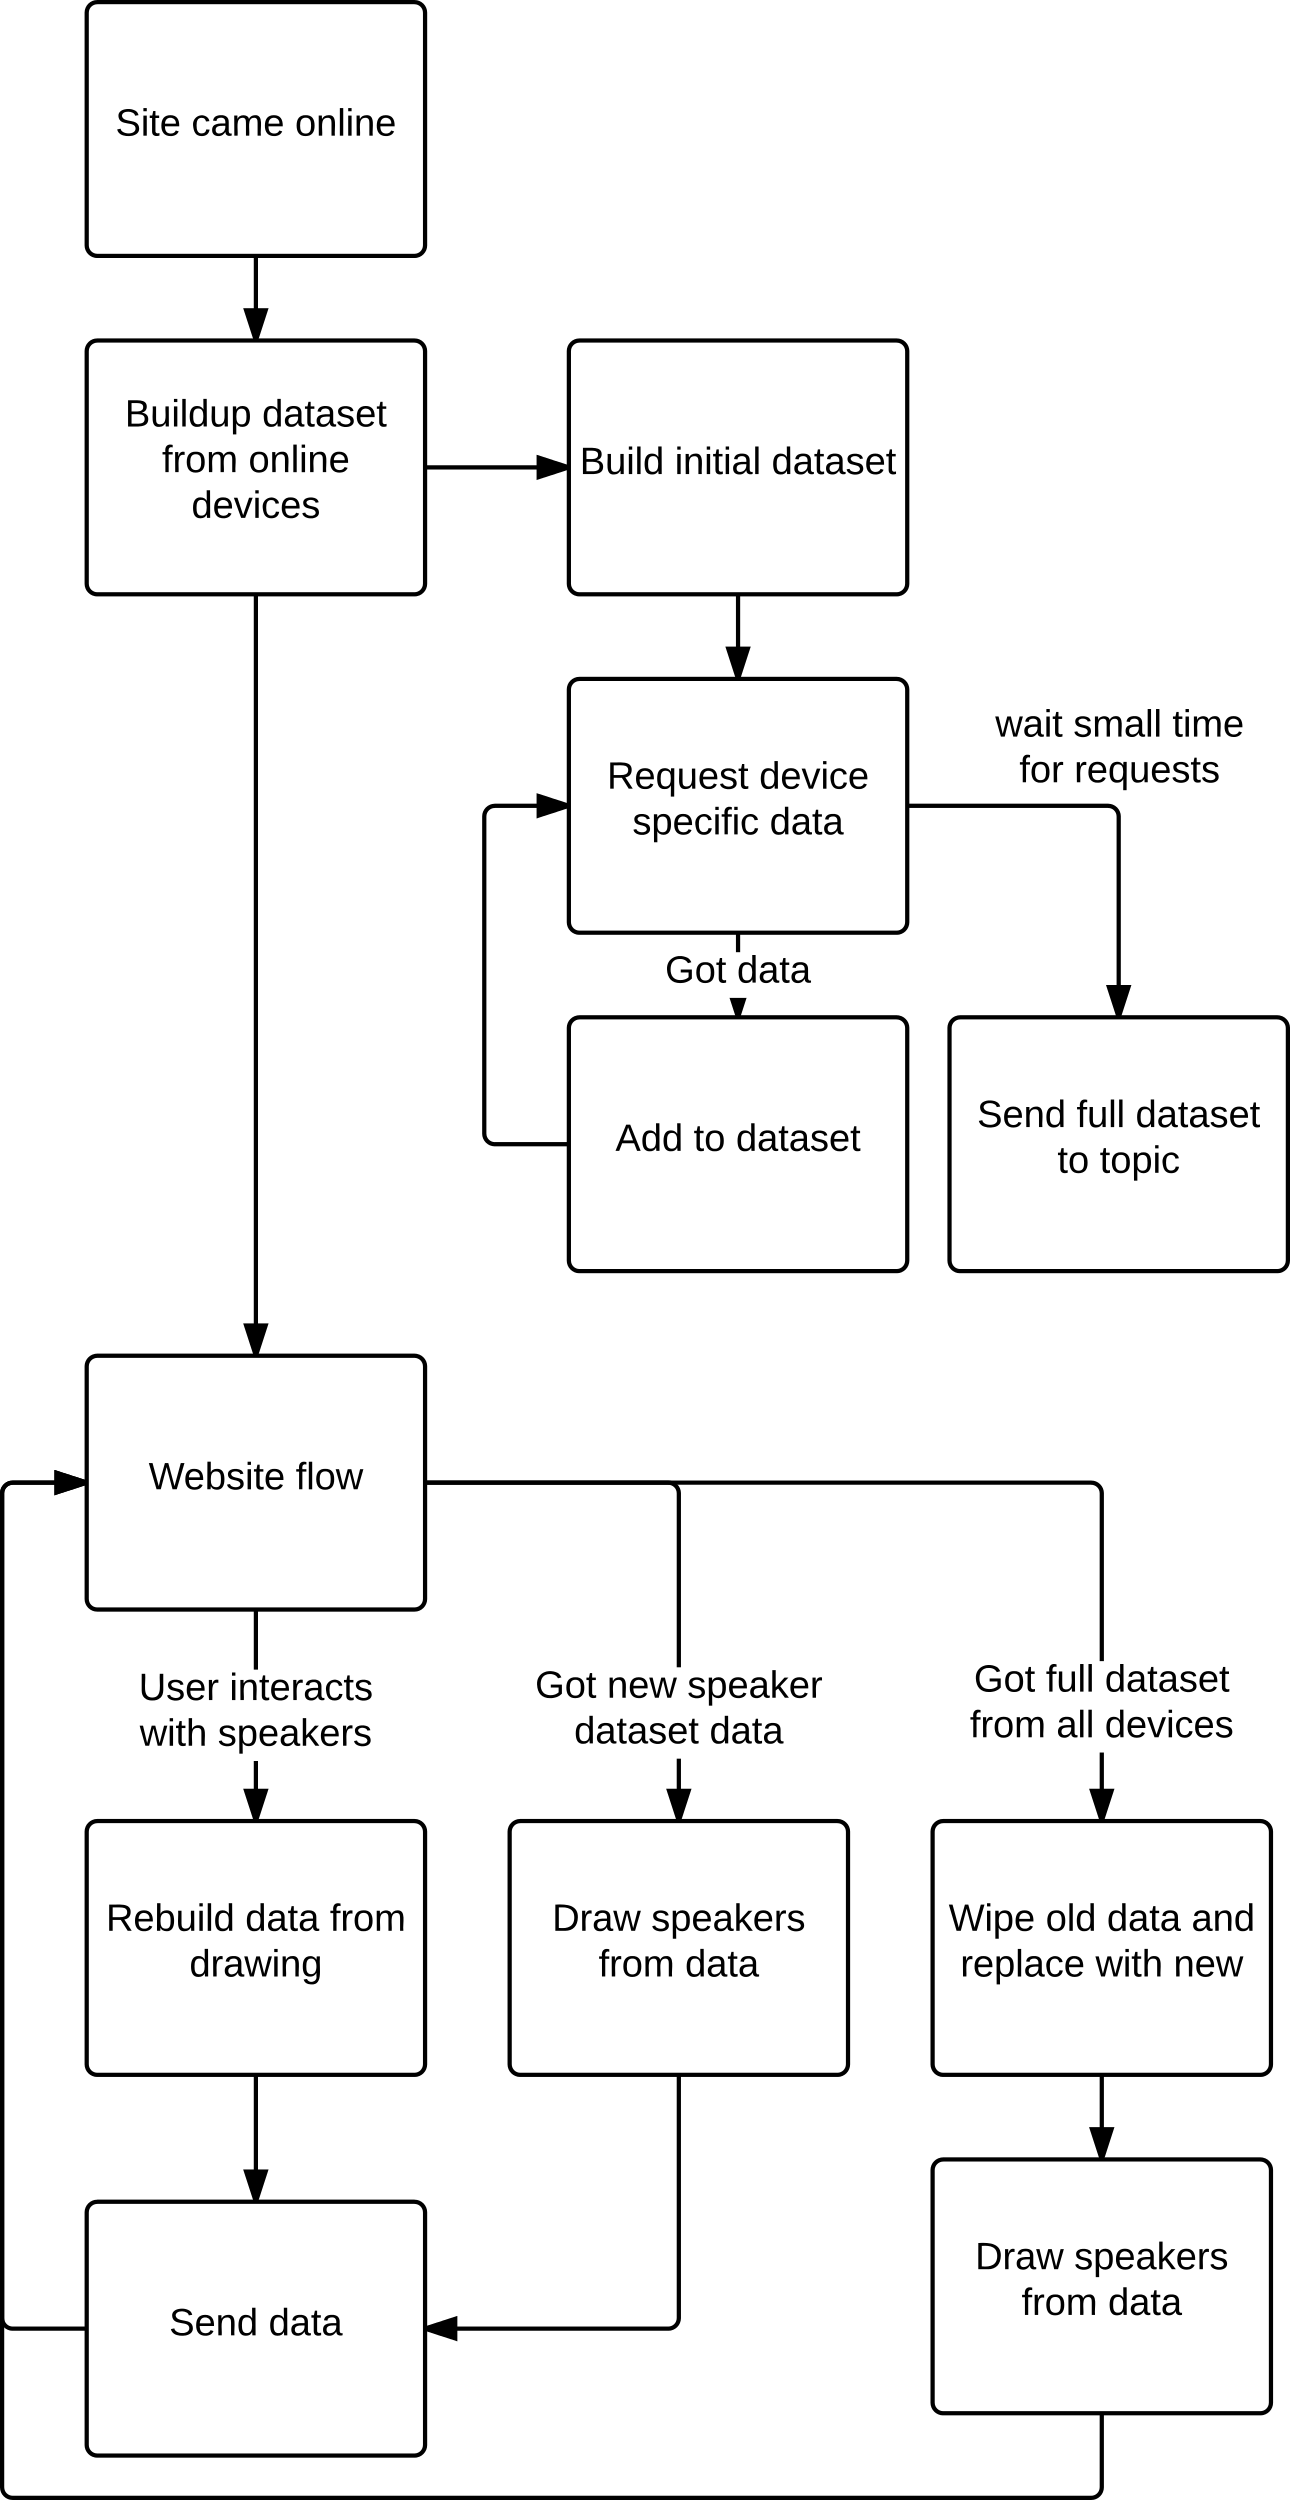
\includegraphics[height=.5\paperheight]{website_flow}
    \caption{The flow of the website}
    \label{fig:website_flow}
\end{figure}

After this initialization, the website is in it's main \textit{"flow"}. From here the site has three possibility's:
\begin{shortlist}
    \item User interacts with the drawing (speakers/objects)
    \item Site got new speaker data (from a single speakers)
    \item Site got complete new dataset
\end{shortlist}
In the \hyperref[chap:Topics]{topics chapter}, are the topics defined that are used to send and receive the data to and from all the devices.

\subsection{Draw and synchronize objects}
To draw and synchronize the drawn speakers/objects, there are three features needed.
One that will draw all the available speakers and objects from the dataset,
one that will generate the dataset from the drawn objects and speakers
and a way of synchronizing this data between website and speaker.

\subsubsection{Draw speakers from data}
To draw the speakers and objects, the dataset is needed. This dataset holds all the data that is needed for the drawing.
This data holds the relations between the speakers and all the objects.
As seen in figure \ref{fig:website_draw_from_data}, it will simply be a looping scheme.
In this diagram, a somewhat crude software architecture is demonstrated.
The drawing is started from an object, and with all the data that is known, the rest is draw.

Because this is a simple 2D field, all the drawn speakers, will contain all the drawn objects.
I.e. if there are two objects(obj1, obj2) and two speakers(sp1, sp2), sp1 will contain the distance and angle from sp1 to obj1 and obj2.
Sp2 in this example will also have this data, not the same values of course, but it will have the distance and angle from sp1 to obj1 and obj2.
With this knowledge, it is only needed to draw an object or speaker once and after that it is not needed to check if the remaining data of that object correlates with the data of other speakers.
In this case, it is assumed that the data represents a single 2D drawing area.

\begin{figure}[H]
    \centering
    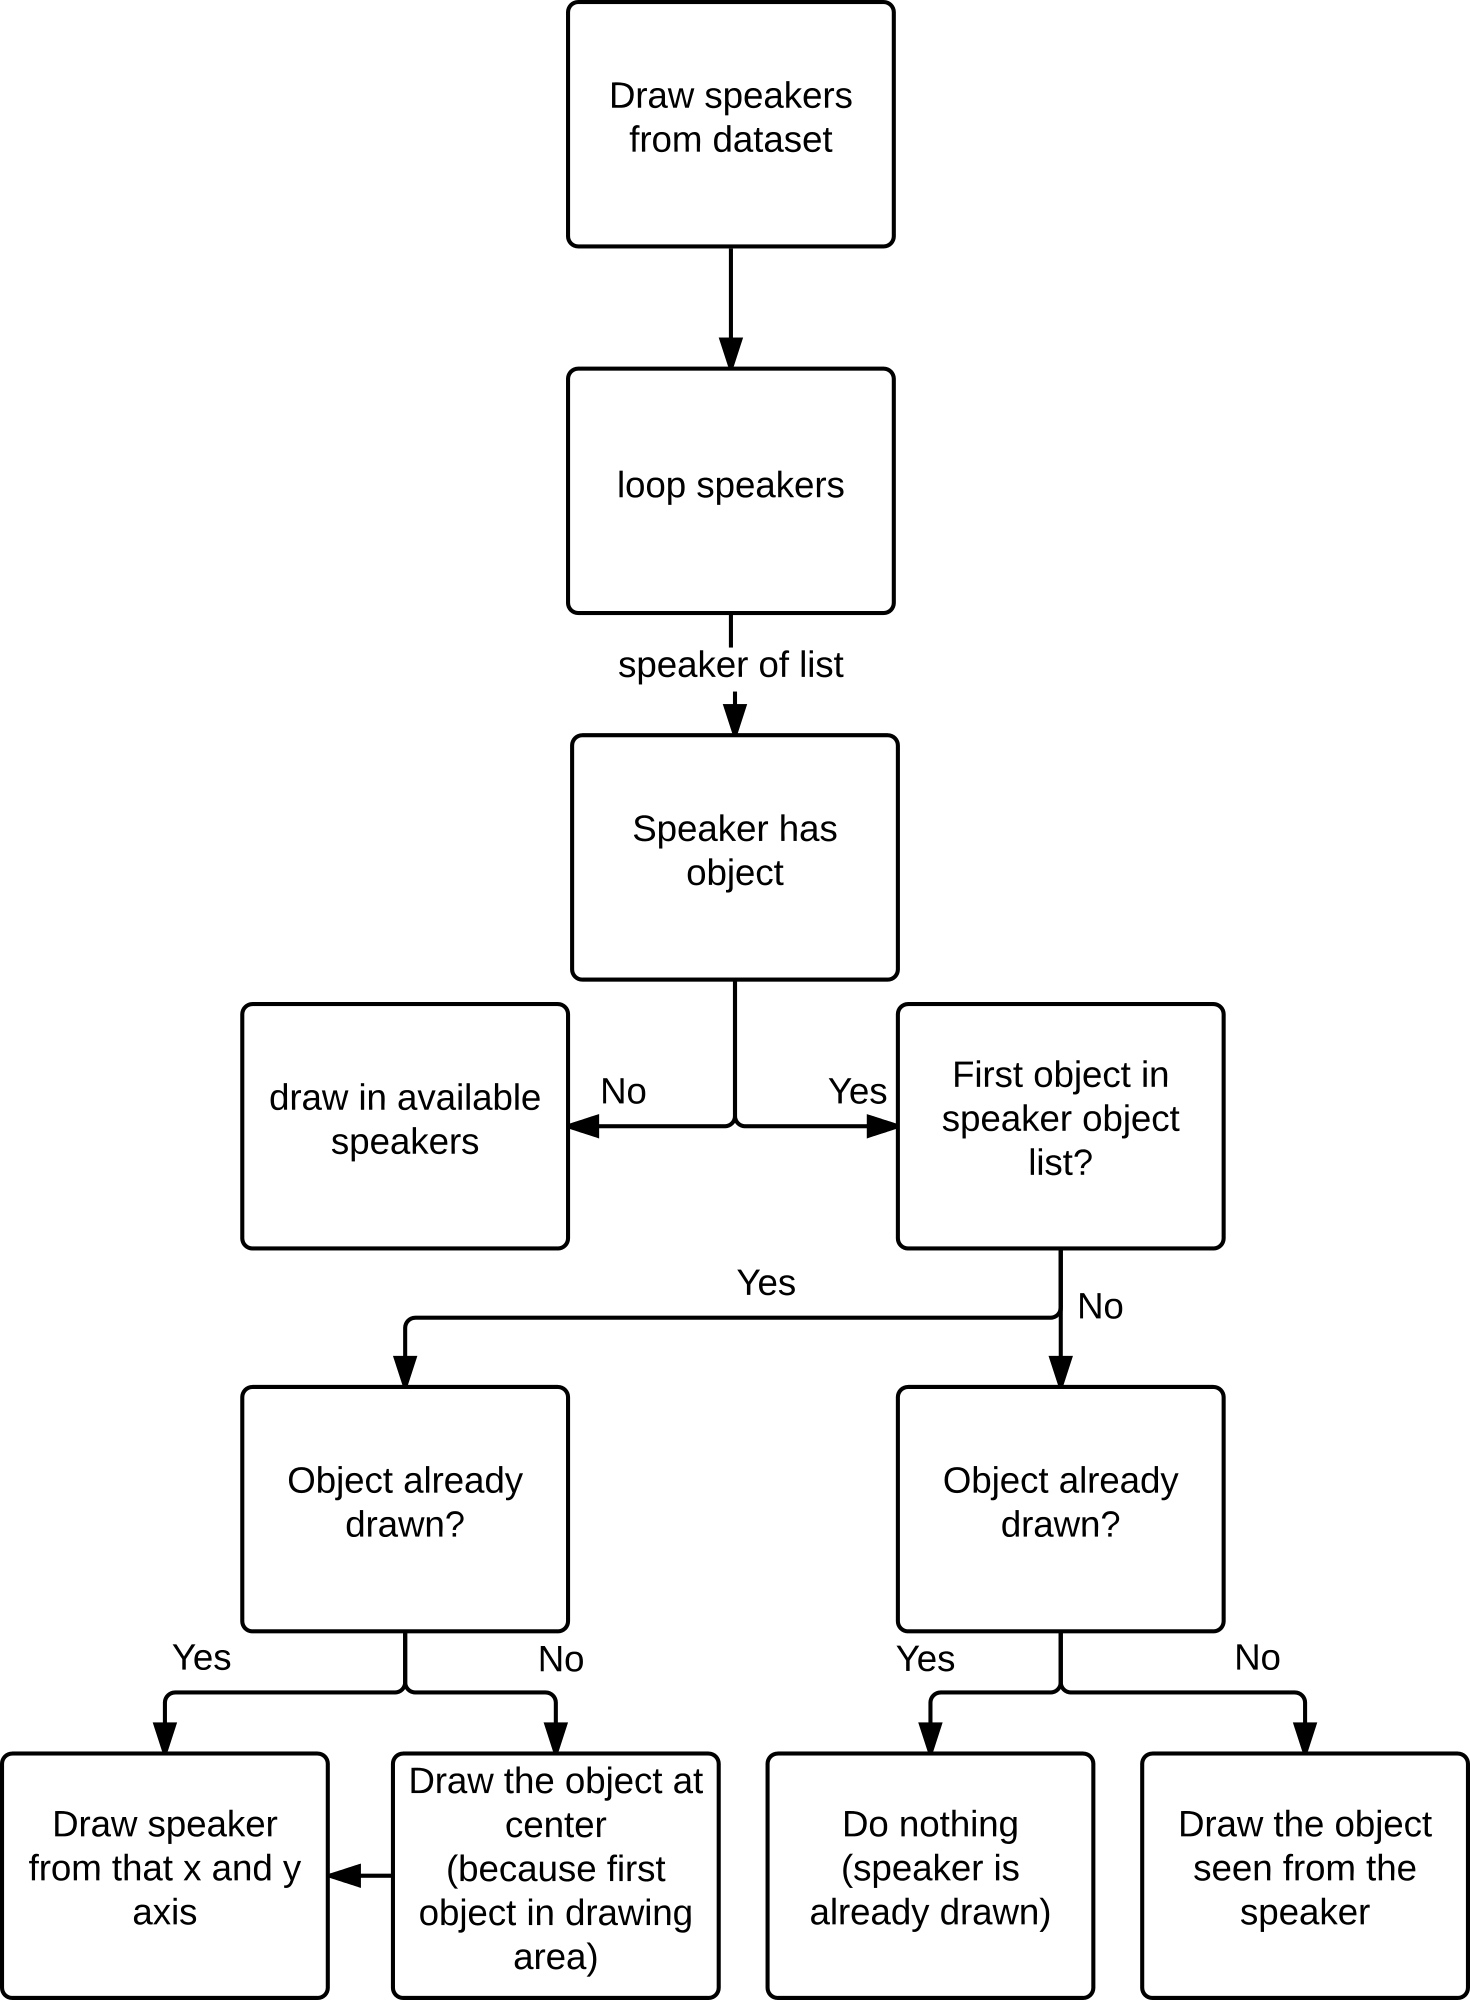
\includegraphics[height=.5\paperheight]{website_draw_from_data}
    \caption{Draw speakers and objects from the dataset}
    \label{fig:website_draw_from_data}
\end{figure}

\subsubsection{Generate dataset from drawing}
This feature has a simple task.
Loop all speakers and calculate all the distances and angles from speaker to the objects.
Figure \ref{fig:website_make_data_from_drawing} describes this quite well.

\begin{figure}[H]
    \centering
    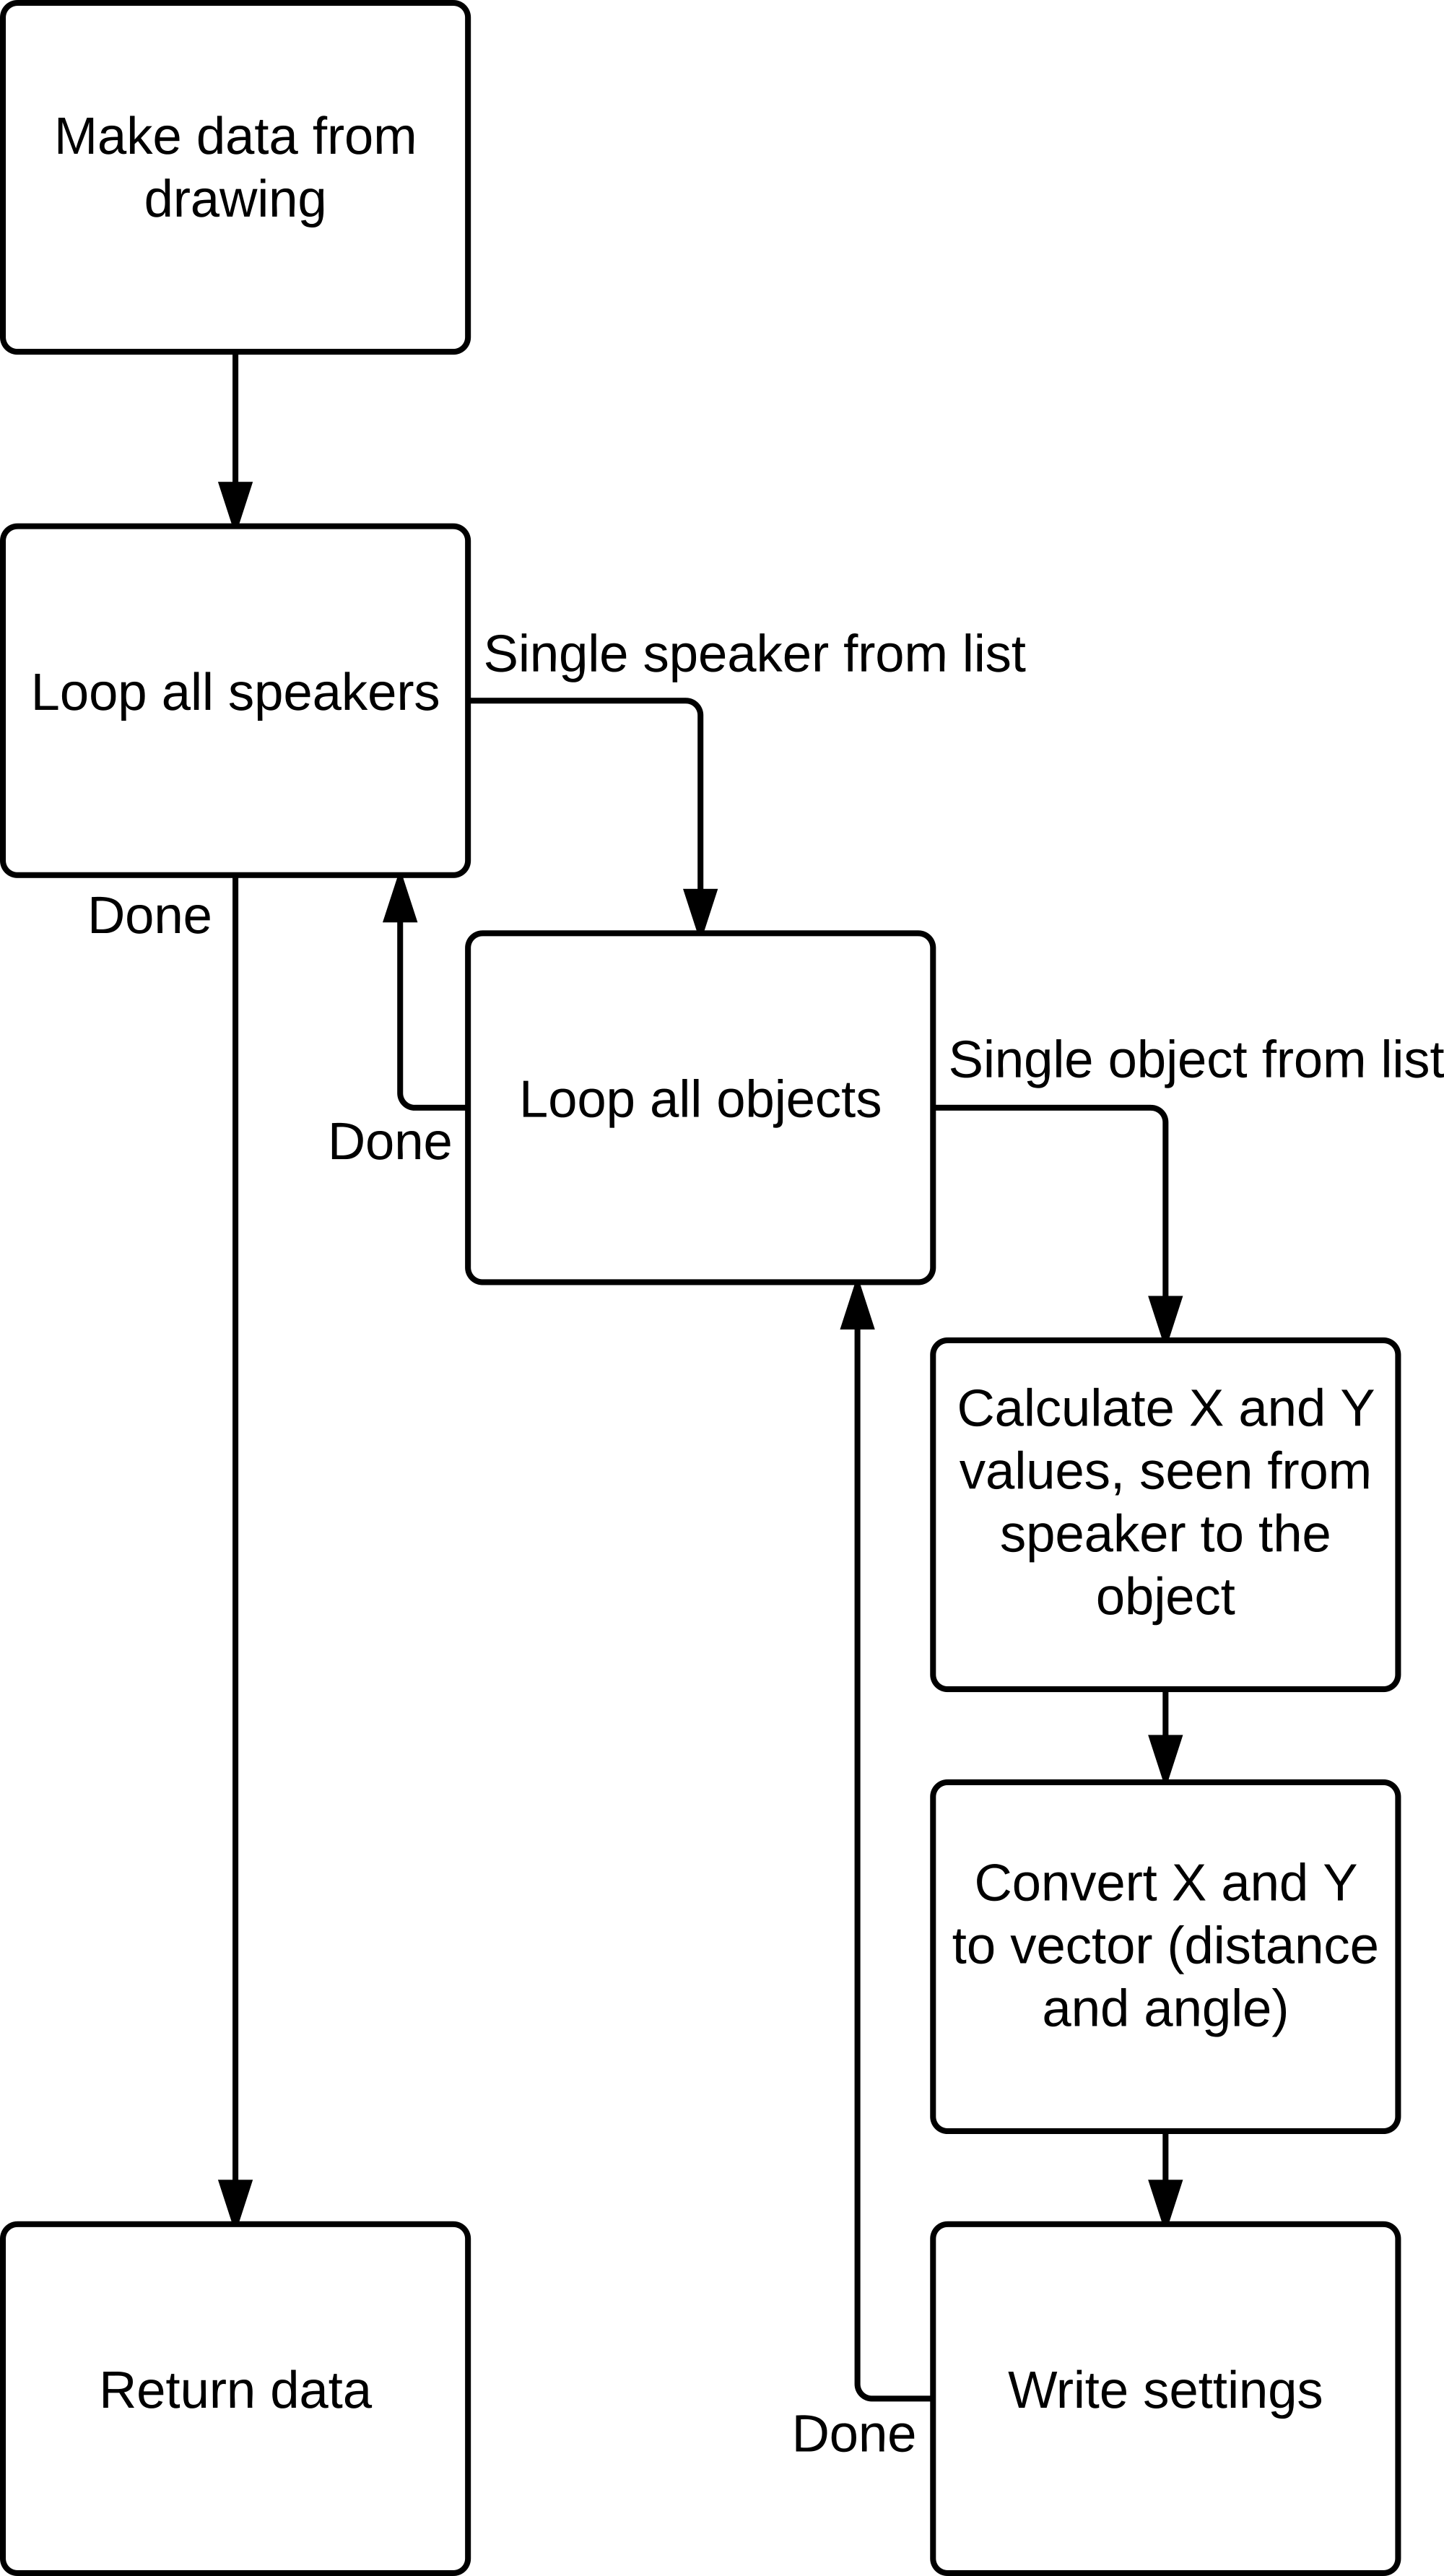
\includegraphics[height=.5\paperheight]{website_make_data_from_drawing}
    \caption{Generate the dataset from the drawing}
    \label{fig:website_make_data_from_drawing}
\end{figure}

\subsubsection{Synchronization}
The last part is the synchronization. This is used for a synchronization between two or more websites and clients.
The dataset is generated.
The moment this is send to a topic for the clients, the other websites however(not the one sending), will also use this data to draw the speakers and objects.
One extra topic is used in this system specific for the website.
The moment, a website sends this data, it also sends the x and y offset of the first drawn object.
This way, the website can redraw the data like it is displayed on the other websites.
This is a reasonable failsafe system with the least amount of overhead.

An other solution would be to send the complete dataset to the clients, but also send one special for the websites.
This second dataset would contain all the speakers and objects and their x and y coordinates.
This means that for x messages to the clients, x messages to the websites needs to be send.
Double the data.
For this reason, making use of the already send dataset and using a small message for the x and y offset of one object is the most practical solution.

Still, this is by no means the best solution.
When that small message with the offset of one object is ignored, all of the drawing will be drawn from the center of the screen instead of the specified x and y offset.
However this is a price that has to be paid.

\subsection{Loading configuration file\\
    \small\nimbus\textit{The not so beautiful approach}}
In this system, a single configuration file is used between website and client.
This file contains all sorts of data.
In JavaScript there is however a problem with this setup. In C or C++ this would be easy, just read it from the local file system.
In general, this is not allowed in JavaScript by design. It's a violation of the sandbox.
There are API's to load a file via a button etc, but this is not user friendly.
Think about it, every time the site is loaded, a window pop's up with the message:
\say{Hello dear user, would you please be kind and load a config file. If you don't, I will not work.}.

The solution was to load this config file on load time. Just like any other JavaScript file is loaded via the script src tags.
The config file was saved with a \say{.js} extension, started with: \say{var CONFIG =} and ended with \say{;}.
The client can filter this out and the website can load in the config file.

It is a solution, maybe not the best, but it works.

\section{Website layout}
In these following paragraphs, the layout and main usage of the site is explained.

\subsection{Idle}
\label{sub:website_idle}
In figure \ref{fig:website_idle} is the state of the website shown when it is in \say{idle} mode.
On the right hand side are the available speakers and objects.
From here, the user can drag these in the draw area.

\begin{figure}[H]
    \centering
    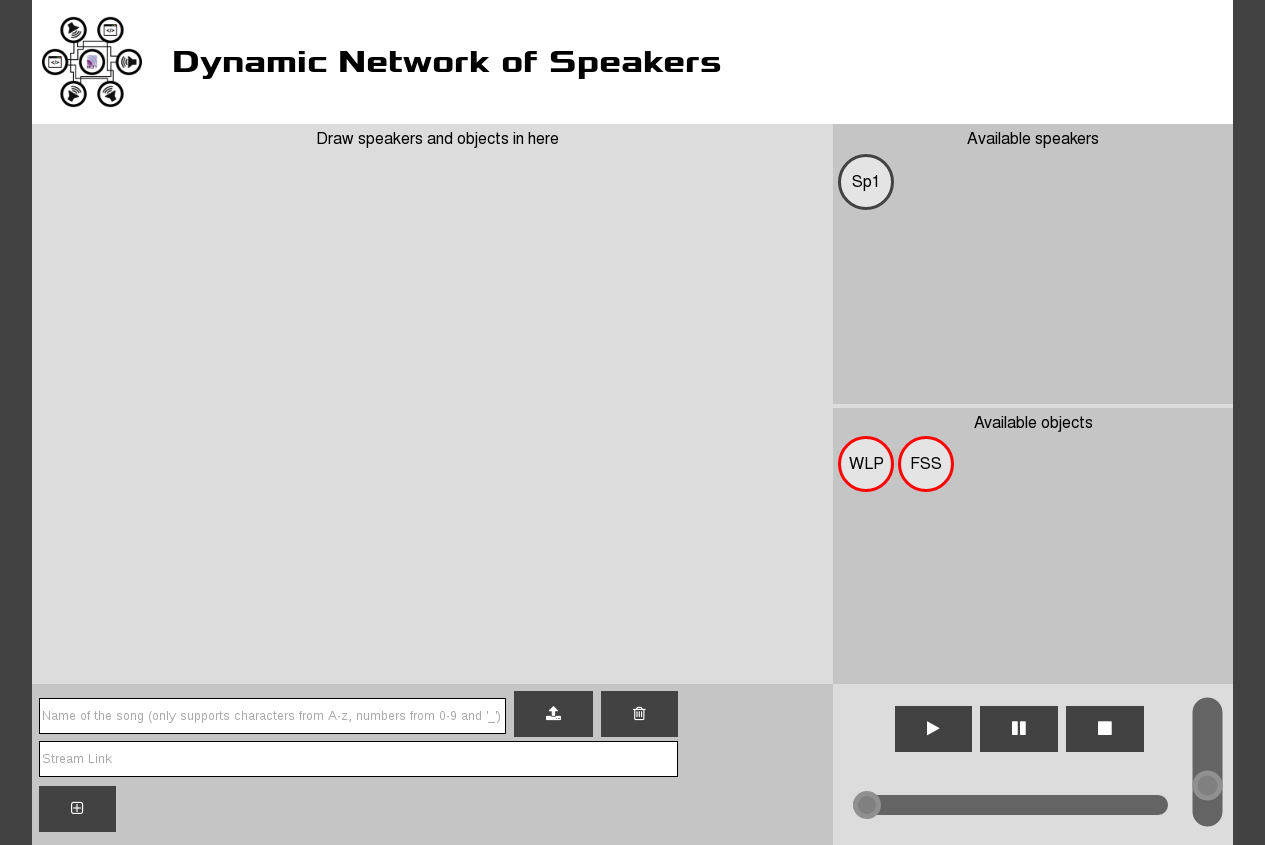
\includegraphics[width=.8\textwidth]{website_idle}
    \caption{Website when idle}
    \label{fig:website_idle}
\end{figure}

The following features are available:
\begin{shortlist}
    \item Available speakers list
    \begin{shortlist}
        \item Listing of all the online speakers
    \end{shortlist}
    \item Available object list
    \begin{shortlist}
        \item Listing off all the available objects
    \end{shortlist}
    \item Music controls (right bottom corner)
    \begin{shortlist}
        \item Music status control (play, pause, stop)
        \item Volume control
        \item Time playback control (not yet implemented)
    \end{shortlist}
    \item Object controls (left bottom corner)
    \begin{shortlist}
        \item Object name field
        \item URI field
        \item Upload button
        \item Delete button
    \end{shortlist}
    \item Extra controls (+ button)
    \begin{shortlist}
        \item See section about the \nameref{sub:website_Extra_options}
    \end{shortlist}
\end{shortlist}

\subsection{Manipulating speakers and objects}
\label{sub:manipulating_speakers_and_objects}
As shown in figure \ref{fig:website_1sp_2obj} and \ref{fig:website_2sp_2obj}, the speakers and objects can be dragged over to the draw area.
In this example there are first one speaker and two objects and in the second example there are two speaker and two objects.
As demonstrated here, the speakers and objects can simply be dragged around via the mouse.

The moment that there is a speaker available, e.g. a speaker comes online, it will show up in it's available speaker list.
From that moment, the user can simply drag the speaker to it's desired location.

\begin{figure}[H]
    \centering
        \begin{minipage}[b]{0.5\textwidth}
            \centering
            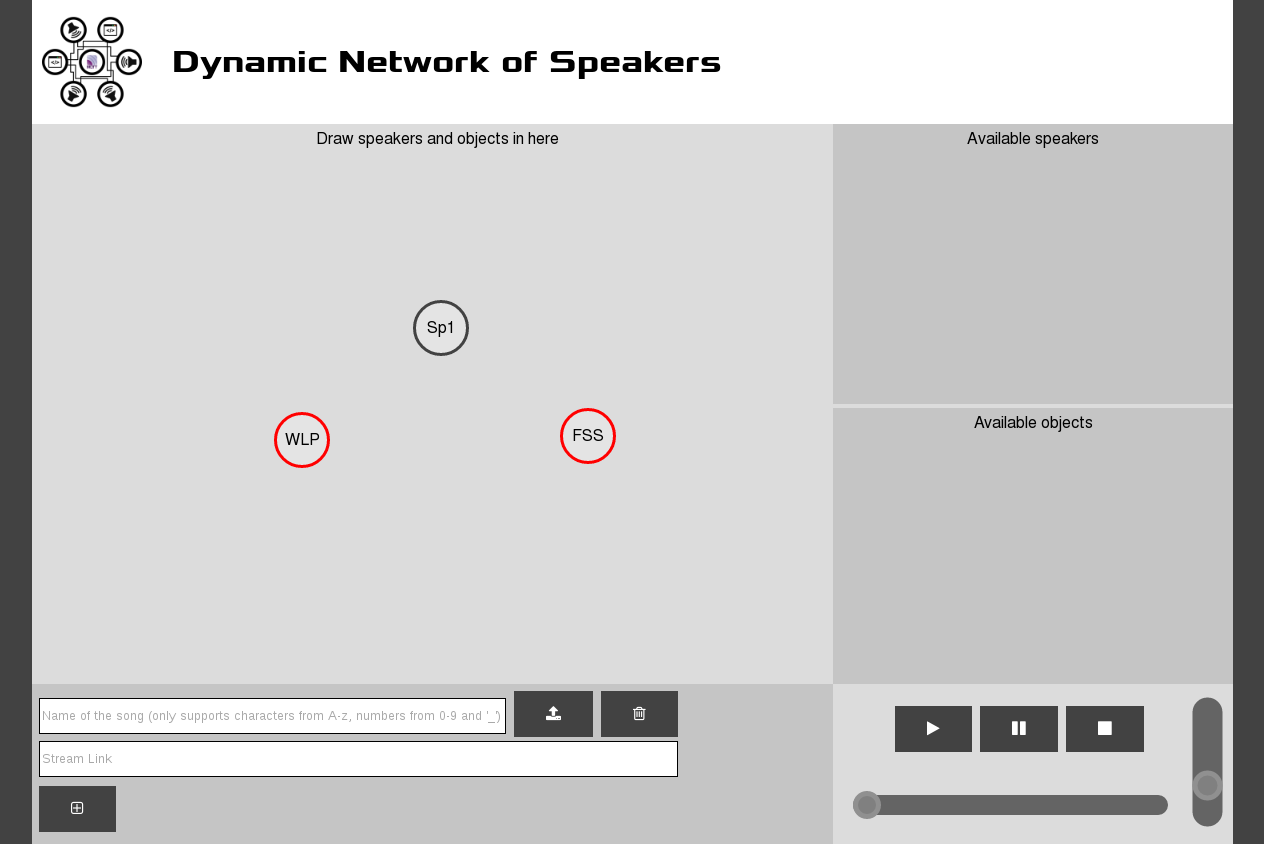
\includegraphics[width=.9\textwidth]{website_1sp_2obj}
            \caption{One speaker and two objects}
            \label{fig:website_1sp_2obj}
        \end{minipage}%
        %
        \begin{minipage}[b]{0.5\textwidth}
            \centering
            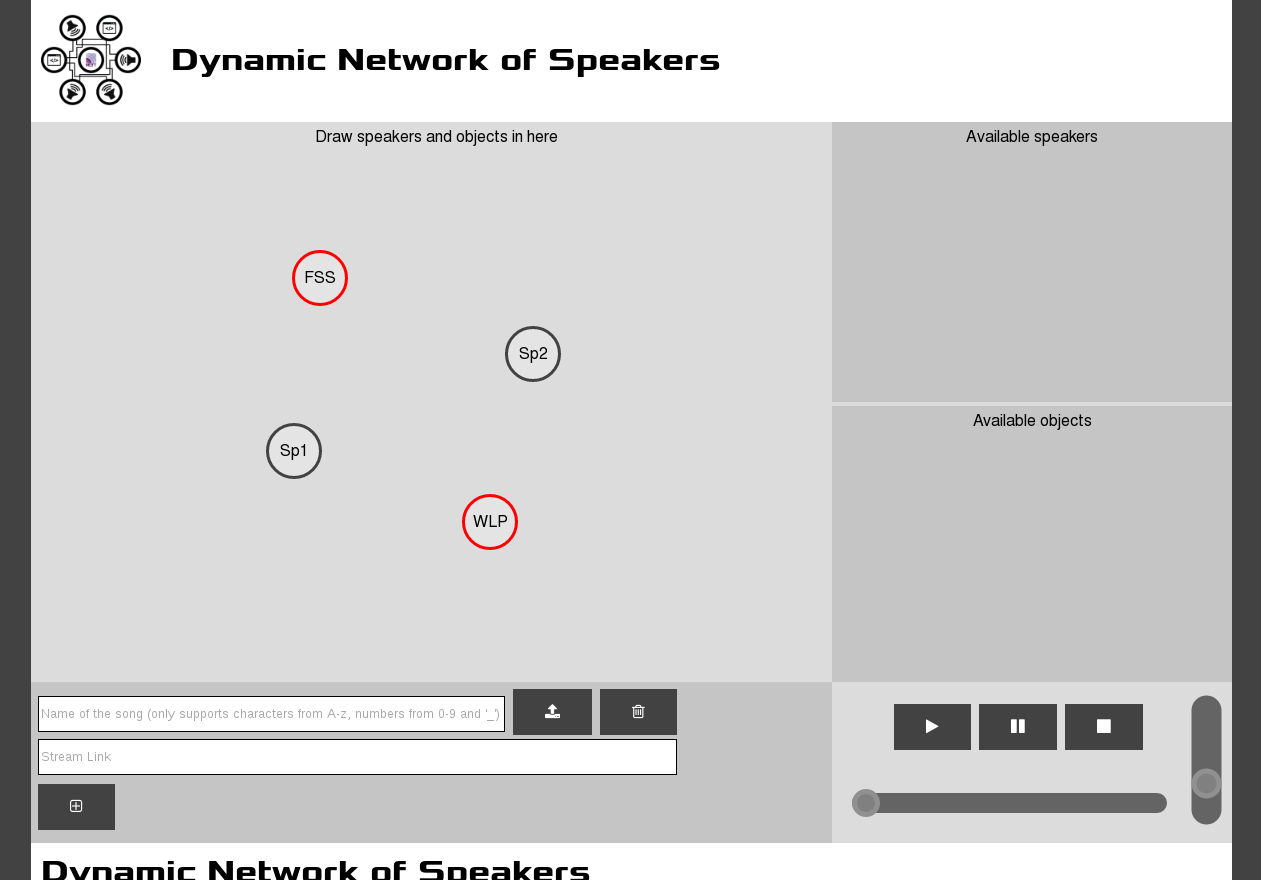
\includegraphics[width=.9\textwidth]{website_2sp_2obj}
            \caption{Two speakers and two objects}
            \label{fig:website_2sp_2obj}
    \end{minipage}
\end{figure}

\subsection{Edit objects}
\label{sub:website_edit_objects}
This website also has the ability to add, delete or modify any existing object.
Figure \ref{fig:website_edit_object} shows this process.

\begin{figure}[H]
    \centering
    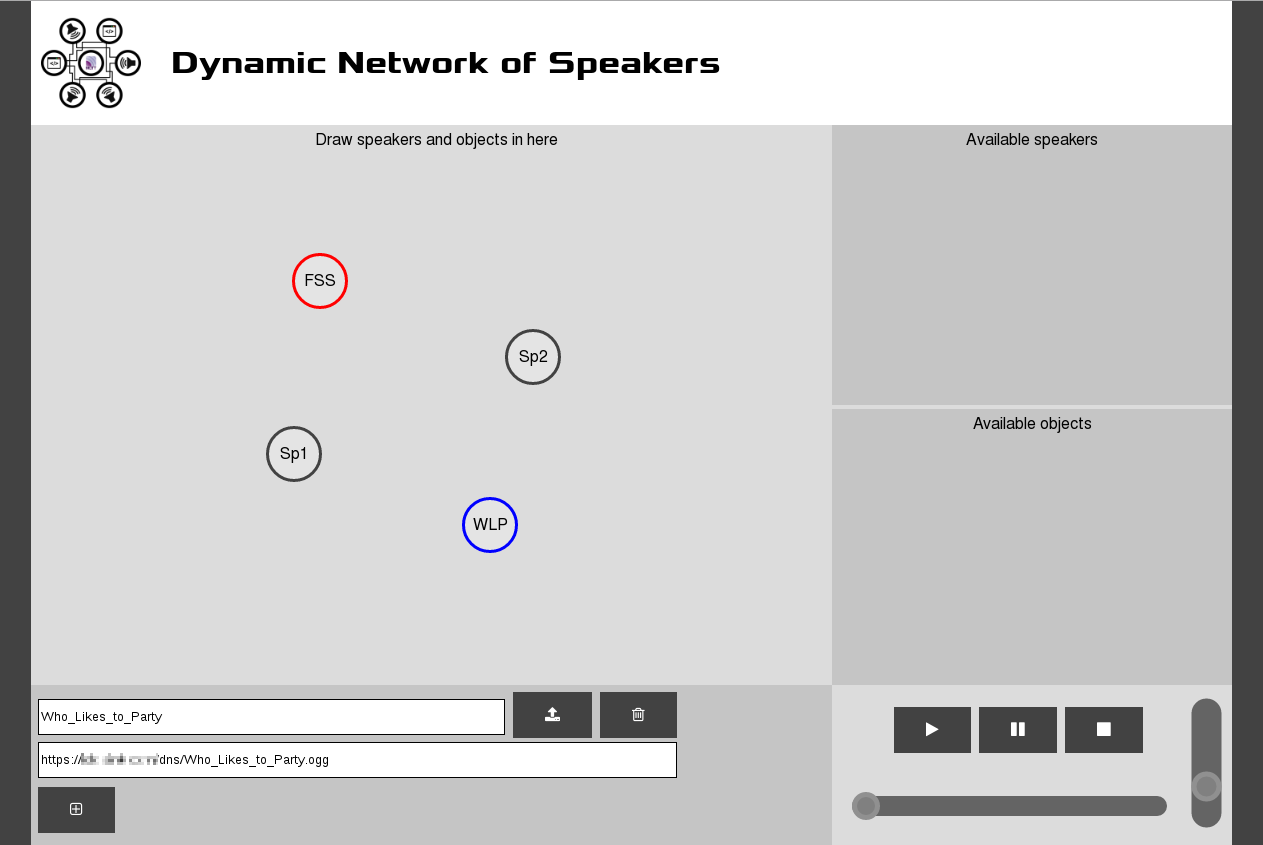
\includegraphics[width=.8\textwidth]{website_edit_object}
    \caption{Edit an object}
    \label{fig:website_edit_object}
\end{figure}

The following list will show the steps necessary to complete the listed action.
\begin{shortlist}
    \item Add an object
    \begin{itemize}
        \item Fill in the Name of the object
        \item Fill in the URI of the object
        \item Press the upload button
    \end{itemize}
    \item Delete an object
    \begin{itemize}
        \item Select an object (the selected object is marked with a colored circle, blue in this case)
        \item Press the delete button
    \end{itemize}
    \item Modify an existing object
    \begin{itemize}
        \item Select an object (the selected object is marked with a colored circle, blue in this case)
        \item Modify the URI\footnote{Editing the name will result in uploading a new object with said name or overriding an object with said name}
        \item Press the upload button
    \end{itemize}
\end{shortlist}

\subsection{Extra options}
\label{sub:website_Extra_options}
The extra options tab, as shown in Figure \ref{fig:website_extra_options}, holds some extra options that are not of a great importance for the main function of this site.

\begin{figure}[H]
    \centering
    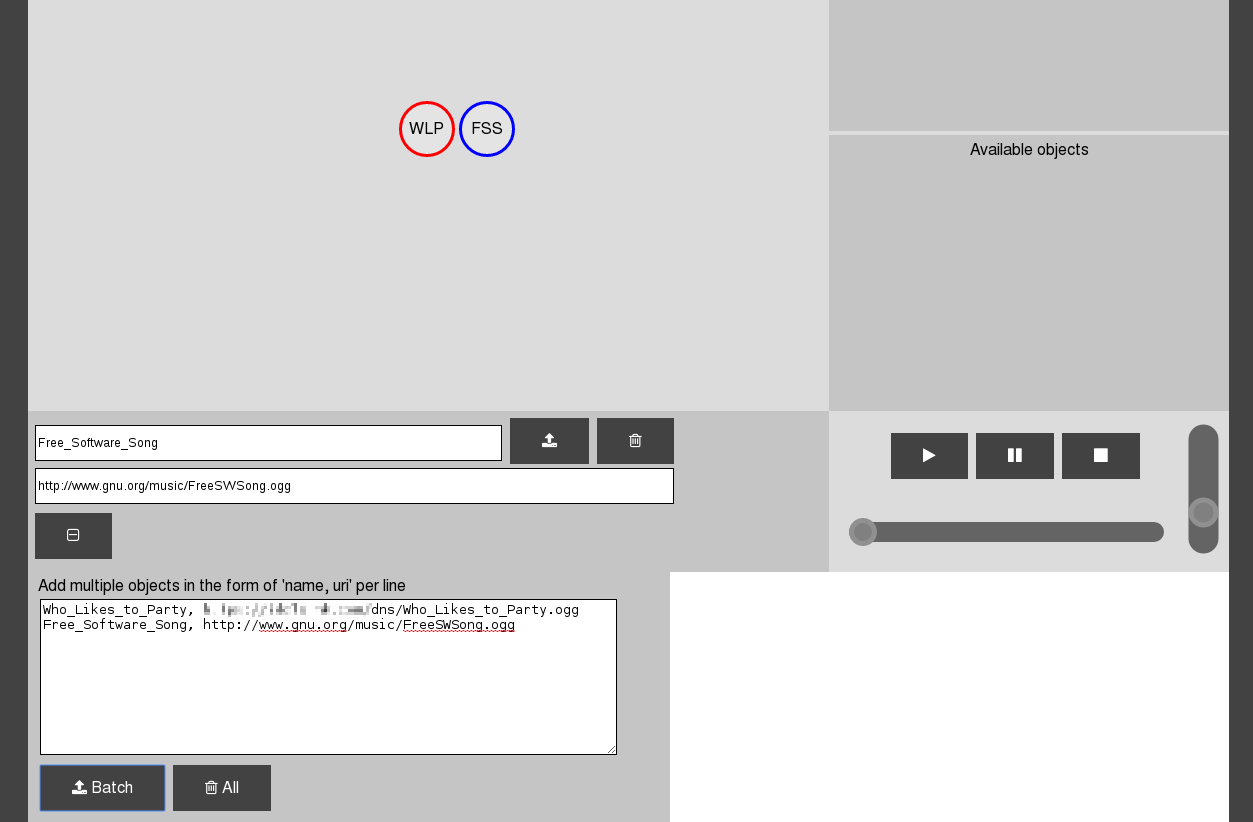
\includegraphics[width=.8\textwidth]{website_extra_options}
    \caption{Extra options}
    \label{fig:website_extra_options}
\end{figure}

This tab has the ability to batch upload and delete all objects.
This can be helpful when using this website in combination with multitrack\footnotemark songs and the user wants to upload multiple objects at once.
\footnotetext{A song split up into multiple stems. A single stem may be delivered in mono, stereo, or in multiple tracks for surround sound.}
